
\documentclass[xcolor=x11names,xcolor=table,compress]{beamer} % handout to disable transitions
%\documentclass[xcolor=x11names,compress]{beamer}

% Many thanks to http://cameron.bracken.bz/beamer-template
%% General document %%%%%%%%%%%%%%%%%%%%%%%%%%%%%%%%%%
\usepackage{graphicx}
%%%%%%%%%%%%%%%%%%%%%%%%%%%%%%%%%%%%%%%%%%%%%%%%%%%%%%


%% Beamer Layout %%%%%%%%%%%%%%%%%%%%%%%%%%%%%%%%%%
\useoutertheme[subsection=false,shadow]{miniframes}
\useinnertheme{default}
\usefonttheme{serif}
\usepackage{palatino}

\setbeamerfont{title like}{shape=\scshape}
\setbeamerfont{frametitle}{shape=\scshape}

\setbeamercolor*{lower separation line head}{bg=DeepSkyBlue4} 
\setbeamercolor*{normal text}{fg=black,bg=white} 
\setbeamercolor*{alerted text}{fg=red} 
\setbeamercolor*{example text}{fg=black} 
\setbeamercolor*{structure}{fg=black} 
 
\setbeamercolor*{palette tertiary}{fg=black,bg=black!10} 
\setbeamercolor*{palette quaternary}{fg=black,bg=black!10} 

\renewcommand{\(}{\begin{columns}}
\renewcommand{\)}{\end{columns}}
\newcommand{\<}[1]{\begin{column}{#1}}
\renewcommand{\>}{\end{column}}
%%%%%%%%%%%%%%%%%%%%%%%%%%%%%%%%%%%%%%%%%%%%%%%%%%



% \usetheme{Malmoe}
% \usetheme{Luebeck}
% \usetheme{Antibes}
% \usecolortheme{rose}
\usepackage{graphicx}
\DeclareGraphicsExtensions{.pdf,.png,.jpg}
\graphicspath{{./images/}}
\usepackage{hyperref}
\usepackage{color}
% ---------------------------------------------------------------------------------------
% Thanks to http://www.guidodiepen.nl/2009/07/creating-latex-beamer-handouts-with-notes/
 % \usepackage{handoutWithNotes}
 % \pgfpagesuselayout{4 on 1 with notes}[a4paper,border shrink=5mm]
 % \pgfpagesuselayout{2 on 1 with notes landscape}[a4paper,border shrink=5mm]
% ---------------------------------------------------------------------------------------

\title{Automata in the Real World (ish)}
\author{Steve Wattam \& \\John Vidler \& \\Maize Contributors}
\institute[2016]{Lancaster University}
\date{\tiny Feb 2016}

\begin{document}

\frame{\titlepage}

\frame{\tableofcontents}

% -----------------------------------------------------------------------------------------
\frame{\frametitle{Aims \& Objectives}
    \begin{itemize}
        \item Context around automata theory
        \vspace{24pt}
        \item<1-> Some experience applying FSMs to algorithmics
    \end{itemize}
}
% tunny: https://c2.staticflickr.com/8/7364/13938027089_6fdd75dd04_b.jpg
%


% -----------------------------------------------------------------------------------------
\section{Automata in Use}
\subsection{Overview}
\frame{\frametitle{Automata in the Real World}
    \begin{itemize}

        \item Automata underpin all of modern computing

        % Without them you'd have specific-use machines
            
        \vspace{10pt}

        \begin{itemize}
                \item Church-turing thesis
                \item Formal proving of systems
                \item Parsing
                \item Functional Programming
        \end{itemize}
        
        \vspace{10pt}

        \item<1-> But they're also useful at a higher level
        % Images for
        %  - biology
        %  - financial analysis
        %  - Industrial control
        %  - Networking 
        %  - Gaming
        % = Anything where a stream needs converting into states or decisions
        
    \end{itemize}
}

\subsection{Cells}
\frame{\frametitle{Cellular Models}
    \begin{itemize}
        \item<1-> Simple rules to model emergent behaviour
        % \item<2-> Lead to chaos theory (Lorenz, Mandelbrot)
    \end{itemize}

    \begin{center}
        \begin{tabular}{|r|c|c|c|c|c|c|c|c|}
            \hline
            \rowcolor[HTML]{EFEFEF} 
            Input                          & 111 & 110 & 101 & 100 & 011 & 010 & 001 & 000 \\ \hline
            \cellcolor[HTML]{EFEFEF}Output & 0   & 1   & 0   & 1   & 1   & 0   & 1   & 0   \\ \hline
        \end{tabular}
    \end{center}


    \begin{center}
        \includegraphics<1>[height=4cm]{lsystem1}
        \includegraphics<2>[height=4cm]{rule90}
        \includegraphics<3->[height=4cm]{lshell}
    \end{center}
}

\subsection{Networking}
\frame{\frametitle{Networking}
    \begin{itemize}

        \item Protocol design heavily uses FSMs
        \item BGP routing:

    \end{itemize}
    

    \begin{center}
        \includegraphics<1>[width=8cm]{bgpfsm}
        \includegraphics<2->[width=8cm]{bgpfsm2}
    \end{center}

    % https://en.wikipedia.org/wiki/Border_Gateway_Protocol#Finite-state_machines
    % Connect state:
    %     - Waits for successful TCP negotiation with peer.
    %     - BGP does not spend much time in this state if the TCP session has been successfully established.
    %     - Sends Open message to peer and changes state to OpenSent.
    %     - If an error occurs, BGP moves to the Active state. Errors are:
    %         - TCP port 179 is not open.
    %         - A random TCP port over 1023 is not open.
    %         - Peer address configured incorrectly on either router.
    %         - AS number configured incorrectly on either router.
    %
}
\frame{\frametitle{Networking}
    \begin{center}
        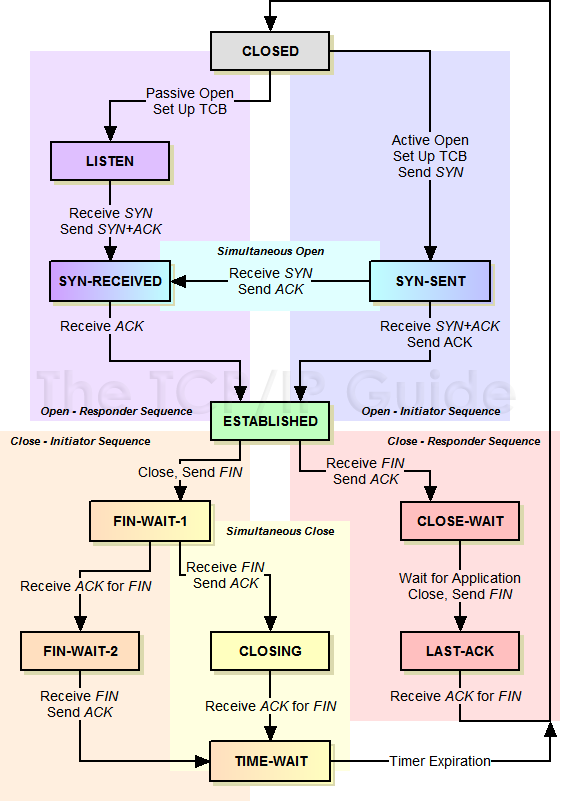
\includegraphics[width=5cm]{tcpfsm}
    \end{center}

    {\tiny \texttt{http://www.tcpipguide.com}}
}

\subsection{Gaming}
\frame{\frametitle{Gaming \& AI}
    \begin{itemize}

        \item Games are essentially one big state machine

        \item Useful for world state and AI
        % The door problem
        % Many libraries for unity, processing etc
        % Fits very well with object-oriented design

    \end{itemize}

    \begin{center}
        \includegraphics<1>[height=4cm]{state-flowchart}
        \includegraphics<2->[height=4cm]{fsm_ant_brain}
    \end{center}
    {\tiny \texttt{http://gameprogrammingpatterns.com/state.html\\
    http://gamedevelopment.tutsplus.com}}
}


% -----------------------------------------------------------------------------------------
\section{Maze Solving}
\subsection{What is a Maze?}
\frame{\frametitle{Know thy Enemy}
\begin{columns} 
    \begin{column}[c]{5cm} 

        \begin{itemize}
            \item<1-> A space with walls
            \item<2-> Has a start and finish (or entrance/exit)
            \item<3-> Stops you from finding your bone

            \item<4-> \textbf{Has some feature making it hard to follow the path}
        \end{itemize}
    \end{column} 
\begin{column}[c]{5cm} 

    \begin{center}
        \includegraphics<3->[width=5cm]{sparky}
    \end{center}

\end{column} 
\end{columns}
}

\subsection{Types of Maze}
\frame{\frametitle{Perfect}
\begin{itemize}
    \item<1-> Has no loops
    \item<2-> Has a route to every point in the maze
\end{itemize}
\begin{center}
    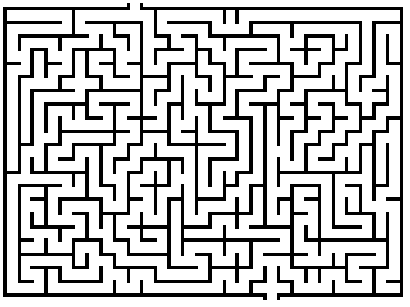
\includegraphics[width=5cm]{perfect}
\end{center}
}
\frame{\frametitle{Braid}
\begin{itemize}
    \item<1-> Has no dead ends, instead using passages that run around and join up again
    \item<2-> Much harder to solve (and generate!)
\end{itemize}
\begin{center}
    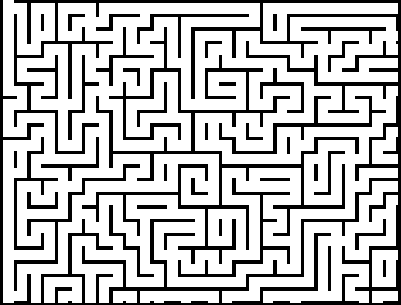
\includegraphics[width=5cm]{braid}
\end{center}
}
\frame{\frametitle{Unicursal}
\begin{itemize}
    \item<1-> Has no junctions, so is a single path
    \item<2-> Sometimes called a labyrinth
    \item<3-> Trivial to solve with automated means
\end{itemize}
\begin{center}
    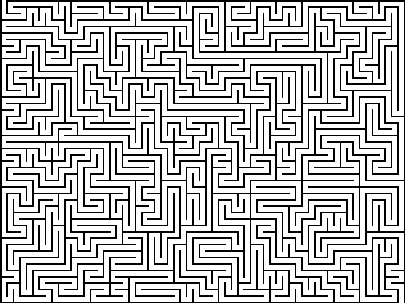
\includegraphics[width=5cm]{unicursal}
\end{center}
}
\frame{\frametitle{Sparse}
\begin{itemize}
    \item<1-> Wide, irregularly-spaced passages.
    \item<2-> Often come in cool designs (not shown here).
\end{itemize}
\begin{center}
    
\includegraphics[width=5cm]{sparse}
\end{center}
}


%\subsection{Properties of Mazes}
%\frame{\frametitle{Properties of Mazes}
%\begin{itemize}
%    \item<1-> \textbf{Bias}---The tendency of a maze to have horizontal or vertical passages.  Makes it hard to go `against the grain'
%    \vspace{15pt}
%    \item<2-> \textbf{Run}---A long, straight, uninterrupted passage
%    \vspace{15pt}
%    \item<3-> \textbf{Elitism}---The ratio of the maze's shortest path against its total path length
%\end{itemize}
%}






% -----------------------------------------------------------------------------------------
\section{Mice}
\subsection{What's one of thems?}
\frame{\frametitle{Mice}

\begin{columns} 
    \begin{column}[c]{8cm} 

\begin{itemize}
    \item<1-> Mice are \textbf{Maze-solving robots}\\
        \visible<2->{\small Mice are also mice}
    \vspace{10pt}
    \item<3-> Compete in many competitions, solving real-life mazes {\tiny (\href{http://www.youtube.com/watch?v=_L9rkLAskWU}{Click me!})}
    \vspace{10pt}
    \item<4-> Limited view of the maze, limited processing power
    \vspace{10pt}
    \item<5-> No awareness of the maze other than what is learned
\end{itemize}

    \end{column} 
\begin{column}[c]{3cm} 

    \begin{center}
        \includegraphics<2->[width=3cm]{mouse1}\\
        \vspace{12pt}
        \includegraphics<1->[width=3cm]{mouse2}
    \end{center}

\end{column} 
\end{columns}
}


\subsection{Abilities \& Limitations}
\frame{\frametitle{Abilities \& Limitations}
\begin{columns} 
    \begin{column}[c]{7cm} 

\begin{itemize}
    \item<1-> Solving a maze is easy, if you can see it all
        \visible<2->{\tiny (\href{http://www.dailymotion.com/video/x43cm2_trapped-in-hedge-maze_fun}{Click me!})}
    \vspace{15pt}
    \item<3-> Mice rely only on pactical real-world input from sensors
    \vspace{15pt}
    \item<4-> So how do they do it? 
\end{itemize}

    \end{column} 
\begin{column}[c]{4cm} 

    \begin{center}
        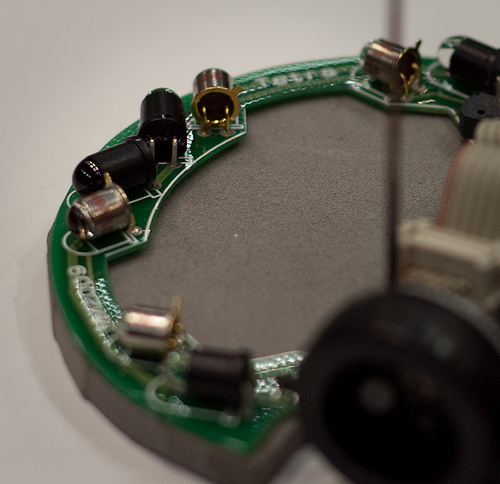
\includegraphics[width=4cm]{mouse3}
    \end{center}

\end{column} 
\end{columns}
}





% -----------------------------------------------------------------------------------------
\section{Control Theory \& Agent-based AI}
\subsection{Overview, Sensing and Actuating}
\frame{\frametitle{Measure--Model--Respond}
\begin{itemize}
    \item<1-> Control theory---each mouse is an `intelligent agent', judging the state of the world from its inputs
    \item<2-> Three basic stages, repeated \textsl{ad infinitum}:
        \begin{enumerate}
            \item<3-> \textbf{Measure} the world about you;
            \item<4-> \textbf{Model} the rest of it to create a virtual world;
            \item<5-> \textbf{Respond} by using information from the model.
        \end{enumerate}
\end{itemize}

\begin{center}
    \includegraphics<3->[width=8cm]{control}
\end{center}

}

\frame{\frametitle{Measure--Model--Respond Problems}
\begin{itemize}
    \item<1-> \textcolor<5->{gray}{Sensors are often inaccurate, or tell us confusing, simple things (data is not information)}
    \item<2-> \textcolor<5->{gray}{The world changes, even when we're not the ones changing it}
    \item<3-> \textcolor<5->{red}{Modelling even simple worlds is difficult!}
    \item<4-> \textcolor<5->{red}{We have to know what to do, even if our model is incomplete}
\end{itemize}
\begin{center}
    \visible<5->{The items in red are all you have to worry about in Maize.}
\end{center}
}


\subsection{Types of Agent}
\frame{\frametitle{Managing the World}
    \begin{itemize}
        \item<1-> \textbf{Stateful/Stateless}---Do we want to remember past events, or treat each sensor reading as a new event?
        \vspace{10pt}
        \item<2-> \textbf{Deterministic/Stochastic}---Do we want to respond in a purely predictable manner?
    \end{itemize}
}
\frame{\frametitle{Inferring State---FSMs}
    \begin{itemize}
        \item<1-> Display how the world \textbf{is}, based on how it \textbf{has changed}
        \item<2-> Can be interrogated without needing new sensor data
        \item<3-> Make transitions between states based on arbitrary, even probabalistic, rules
    \end{itemize}

\begin{center}
    \includegraphics<3->[width=8cm]{fsm}
\end{center}
}
\frame{\frametitle{Determinism}
    \begin{itemize}
        \item<1-> Given the same (sequence of) input, will \textbf{always} produce the same output
        \vspace{10pt}
        \item<2-> Very reliable\\
            \visible<3->{\small but also reliably bad if the rules are poor}
        \vspace{10pt}
        \item<4-> Nondeterminism can involve fuzzy logic, probability, or guesswork\\
            \visible<5->{\small Closer to human judgement, but very hard to get `just right'}
    \end{itemize}
}
\frame{\frametitle{Demos}
    \begin{itemize}
        \item<1-> Deterministic vs. Stochastic
        \begin{itemize}
            \item<2-> DaveBot is (entirely) stochastic, has no rules
            \item<2-> LeftBot is deterministic, has only rules
            \item<2-> Gorad (v2) makes random decisions when it has no rules to fall back on
        \end{itemize}

        \vspace{10pt}
        \item<3-> Stateful vs. Stateless
        \begin{itemize}
            \item<4-> LeftStateBot is stateful, remembers a long sequence of actions
            \item<4-> LeftBot is not
            \item<4-> GraphBot is \textbf{very} stateful
        \end{itemize}
    \end{itemize}
}

\subsection{Complexity}
\frame{\frametitle{Complexity of Maze Solving}
    \begin{itemize}
        \item<1-> Algorithmically, the best solution to a maze is to choose the best right path each time:\\
            \textcolor<2->{red}{The maze is just a big tree of right/wrong choices}
        \vspace{10pt}
        \item<3-> The best case is thus equivalent to a binary search, plus the time needed to move
        \vspace{10pt}
        \item<4-> This becomes $O(n log_2 n)$, where $n$ is the number of choices.% (plus a bit of time to travel from start to finish).
    \end{itemize}
}




% -----------------------------------------------------------------------------------------
\section{Introduction to Maize}
\subsection{The Framework}
\frame{\frametitle{Overview}
    \begin{itemize}
        \item<1-> Manages \texttt{Bot}s and \texttt{Maze}s, and simulates a virtual world
        \vspace{5pt}
        \item<2-> Tile-based discrete environment
        \vspace{5pt}
        \item<3-> A tile can be a start, finish, space, or wall
    \end{itemize}

    \vspace{5pt}
    \begin{center}
        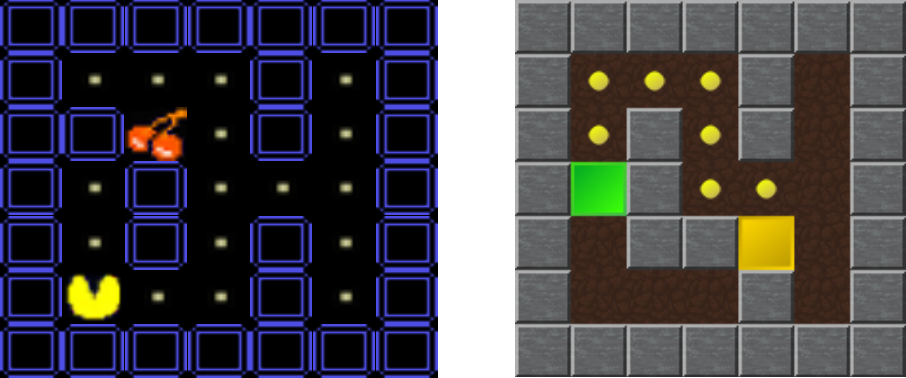
\includegraphics[width=7cm]{mazepic1}
    \end{center}
}
\frame{\frametitle{The Life of a Bot}
    \begin{itemize}
        \item<1-> Bots can only see one block ahead:
            \begin{itemize}
                \item<2-> Their immediate surroundings (3x3 array around them)
            \end{itemize}\\
    
            
        \vspace{5pt}
        \begin{center}
            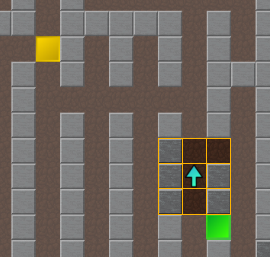
\includegraphics[width=5cm]{context1}
        \end{center}

        \vspace{7pt}
    \item<7-> Bots can move only \textbf{one tile per `tick'}, and only \textbf{\textcolor{red}{L}eft}, \textbf{\textcolor{red}{R}ight}, \textbf{\textcolor{red}{F}orward} and \textbf{\textcolor{red}{B}ack}
        % \item<8-> Each move has a time limit (bots are considered `stuck' if they hit this a lot)
    \end{itemize}
}
\frame{\frametitle{FSM Bots}
    \begin{itemize}
        \item Four ``Special'' States: F, B, L, R.
        \item Boolean expressions control each edge
        \item Other states are ignored
    \end{itemize}

    \vspace{5pt}
    \begin{center}
        
\includegraphics[width=8cm,height=4cm]{botfsm1}
    \end{center}
}
\subsection{Code Introduction}
\frame{\frametitle{Demo, Code Rundown}
    \begin{center}
        A quick overview of the bots we have\\
        \vspace{10pt}
        \url{http://stephenwattam.com/projects/maize/}
    \end{center}
}
% -----------------------------------------------------------------------------------------

\frame{\frametitle{Fin}
    \begin{center}
        All resources available from\\
        \vspace{10pt}
        \url{http://stephenwattam.com/teaching/maize/}
    \end{center}
}


% -----------------------------------------------------------------------------------------
\end{document}
